
\documentclass[12]{article}
\usepackage[utf8]{inputenc}
\usepackage{cite}
\author{par4111 \\ Adrià Cabeza, Xavier Lacasa \\ Departament d' Arquitectura de Computadors}
\title{Lab 3: Embarrassingly parallelism with OpenMP: Mandelbrot set }
\date{\today \\ 2018 - 19 SPRING}
\usepackage{graphicx}
%\usepackage[left=3.5cm, right=3.5cm]{geometry}
\usepackage{subcaption}
\usepackage{pgfplots}
\usepackage{listings}
\usepackage{xcolor}
\usepackage{float}
\lstset{
  basicstyle=\ttfamily,
  showstringspaces=false,
  commentstyle=\color{orange},
  keywordstyle=\color{blue},
	frame=tb,language=C,breaklines=true,numbers=none,  stringstyle=\color{red}, tabsize=3,   showstringspaces=false,
  columns=flexible, 
}
\begin{document}
\maketitle

\vspace*{\fill}
\begin{center}

\includegraphics[scale=0.5]{images/UPClogo.png}
\end{center}
\newpage
\tableofcontents
\newpage
\section{Introduction}

This second laboratory assigment consists on a series of tests and modifications on a program called Mandelbrot. The program computes a particular set of points belongig to the complex domain,whose boundary generates a distinctive and recognisable two-dimensional fractal shape.

\section{Task decomposition and granularity analysis}
In this section we will explain the different task decomposition strategies and granularities explored using Tareador and the Mandolbrot program. 


\textbf{Which are the two most important common characteristics of the task graphs generated for the two task granularities (Row and Point) for the non-graphical version of mandel-tareador? Obtain the task graphs that are generated in both cases for -w 8.
}

Firstly, we will do a task at each single point (row,col) level. Please look at the Figure \ref{point} to see the dependency graph obtained at that level of granularity. 

\begin{figure}[H]
\centering
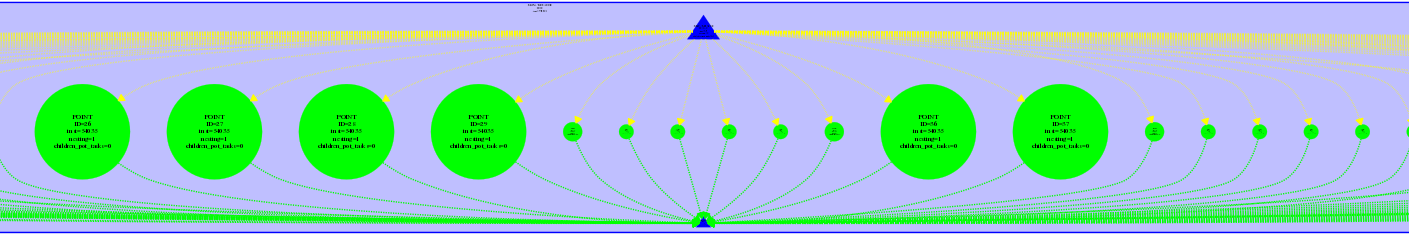
\includegraphics[scale=0.25]{images/point_dependencygraph.png}
\label{point}
\caption{Part of the dependency graph for point decomposition}
\end{figure}

The second one consists on doing the tasks at the row level. Please look at the Figure \ref{Row} to see the dependency graph obtained at that level of granularity. 


\begin{figure}[H]
\centering
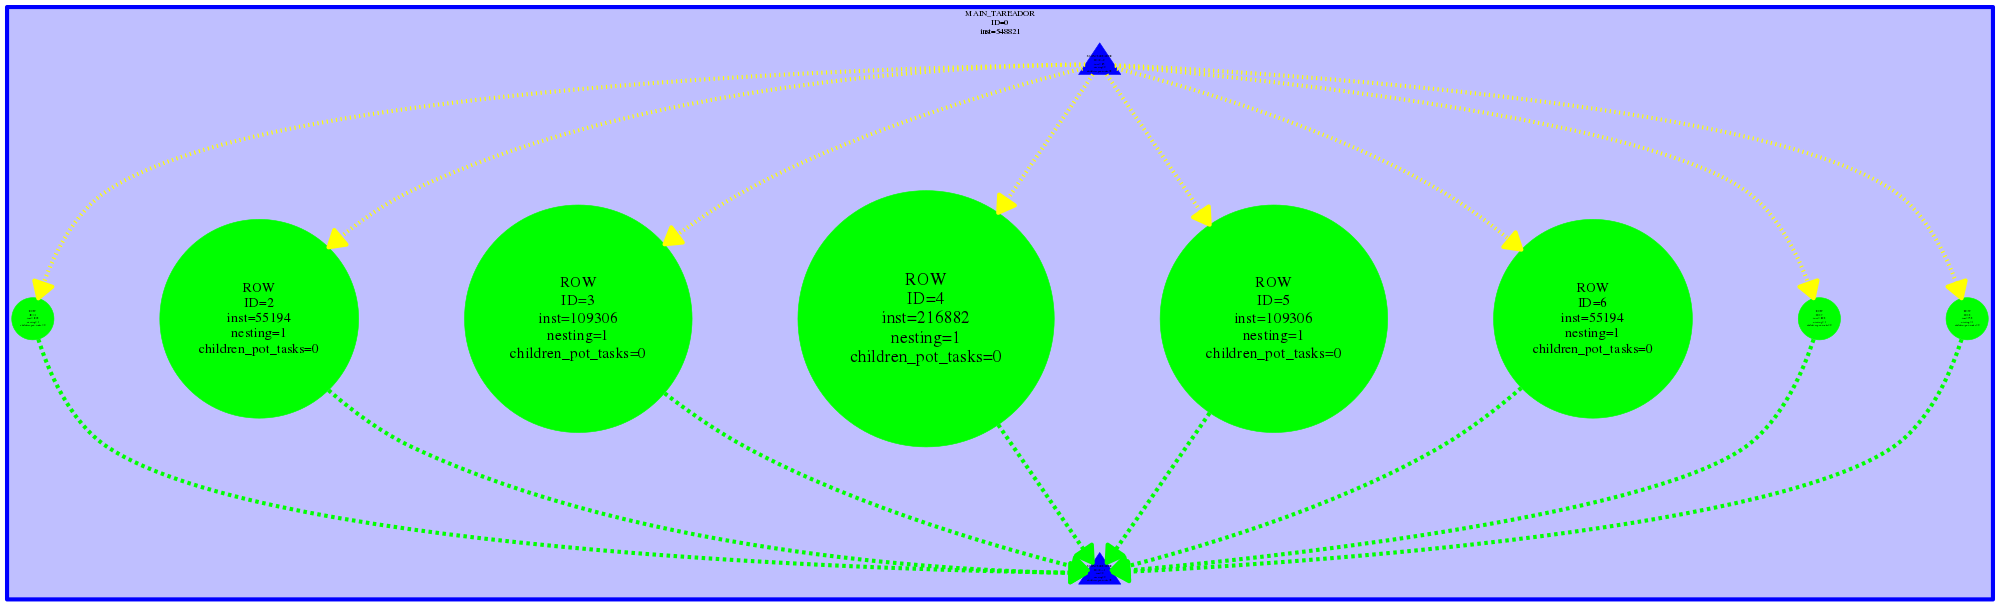
\includegraphics[scale=0.2]{images/row_dependencygraph.png}
\label{Row}
\caption{Dependency graph for point decomposition}
\end{figure}


If we compare each dependency graph we can observe that the load between different tasks is not equally distributed: the sizes of the tasks have very different values. For this reason we decided that to create tasks in the \textit{static mode} is not the best option. We should use \textit{dynamic mode} instead. Also we can observe that there is no shared data between tasks so there are no dependencies. 


\textbf{Which section of the code is causing the serialization of all tasks in mandeld-tareador? How do you plan to protect this section of code in the parallel OpenMP code?
}

The previous analysis was made using the \textit{mandel-tar} program which does not show the fractal on the screen. If we analyse the program that shows the image (\textit{mandeld-tar}, we get the following dependency graph (Figure \ref{graphic}).


\begin{figure}[H]
\centering
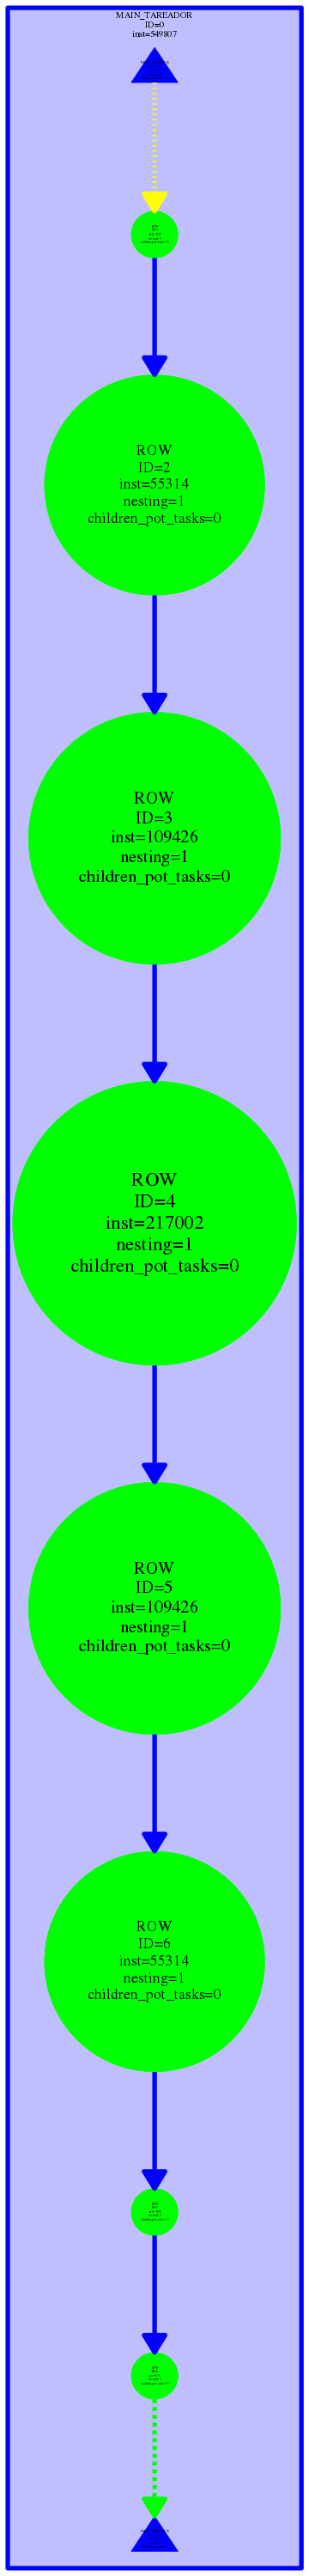
\includegraphics[scale=0.2]{images/dependency_graph_Mandeld.png}
\label{graphic}
\caption{Dependency graph for \textit{mandeld} program}
\end{figure}

It is easy to conclude that we have obtained a sequential version of the program with a lot of dependencies that do not allow to parallelize. The reason for this behaviour is the way the results are printed in the screen (we need to print the dots line by line so parallelism is useless here). In order to parallelize the code we should modify it as follows: 
\begin{lstlisting}[frame=single]
#pragma omp critical
{
	XSetForeground(display,gc,color);
	XDrawPoint(display,win,gc,col,row);
}
\end{lstlisting}


%
%WE HAVE TO REMEMBER THAT THE DEPENDENCY IS DUE TO THE WINDOWS THAT IS USED TO DRAW THE MANDELBROT SET (X11)
%
%\textbf{ADD THE MISSING PRAGMA}, WE NEED TO CREATE A CRITICAL SECTION TO AVOID THE VARIABLE ACCESS THAT CREATES THE CONFLICT IN ORDER TO AVOID THE POSSIBLE DATA RACE (IT IS A VARIABLE OF THE X11 SECTION). 
%we need to add a frame with the code
%
%%ES IMPORTANT FICAR-HO JUNT!
%OMP_NUM_THREADS= 8 ./mandel-omp -i 10000 -o 
%
%OMP_NUM_THREADS= 1 ./mandel-omp -i 10000 -o 






\end{document}